% Cap�tulo 2
\chapter{Avaliação de Soluções para Resolver o Cubo de Rubik}

O cubo de Rubik é considerado um dos quebra-cabeças mais bem-sucedidos de toda história. Isto se deve, principalmente, ao fato de ter mais de 350 milhões de unidades vendidas para o mundo todo. 


\begin{quotation}
(...) Aproximadamente uma em cada sete pessoas já brincaram com o quebra-cabeça. Este pequeno cubo de seis cores passou a representar uma década. Ele apareceu em obras de arte, vídeos famosos, filmes de Hollywood e até teve o seu próprio programa de TV, ele representava tanto genialidade quanto confusão, deu início a um novo esporte (speedcubing) (...) \cite{alecio}.
\end{quotation}


O cubo mágico surgiu em 1974 quando Erno Rubik, professor universitário de design de interiores, teve a ideia de construir um cubo capaz de rotacionar suas faces para que pudesse ilustrar melhor para seus alunos o conceito tridimensional \cite{luis}. O primeiro exemplar era de madeira e cada uma das seis faces do cubo era pintada de uma cor diferente, sendo inspirado por outro quebra-cabeça chamado Tangram. O próprio criador do cubo demorou cerca de um mês para remontá-lo na configuração inicial \cite{luis}.


\begin{quotation}
Matemáticos ajudaram a divulgar o cubo mágico apresentando-o em conferências internacionais e o levaram a uma feira de brinquedos em Nuremberg em 1979, daí o destino dos cubos mágicos mudou para sempre. Nesta feira, os cubos encantaram os participantes e também um especialista no mundo dos brinquedos, Tom Kremer, que concordou em distribuir e comercializar em todo o mundo o brinquedo através de uma pequena empresa chamada Toy Company estabelecendo desde então um novo nome para o produto: "Cubo de Rubik", em homenagem ao seu inventor \cite{jose}.
\end{quotation}


Diversos entusiastas do brinquedo continuam produzindo puzzles baseados no cubo de Rubik, como o Megaminx (dodecaedro), Pyraminx (tetraedro) e o cubo 2x2x2 (variação do tradicional cubo 3x3x3), como mostra a Figura \ref{fig:figPuzzles}.

\begin{figure}[!htb]
    \centering
    \subfloat[Megaminx]{
        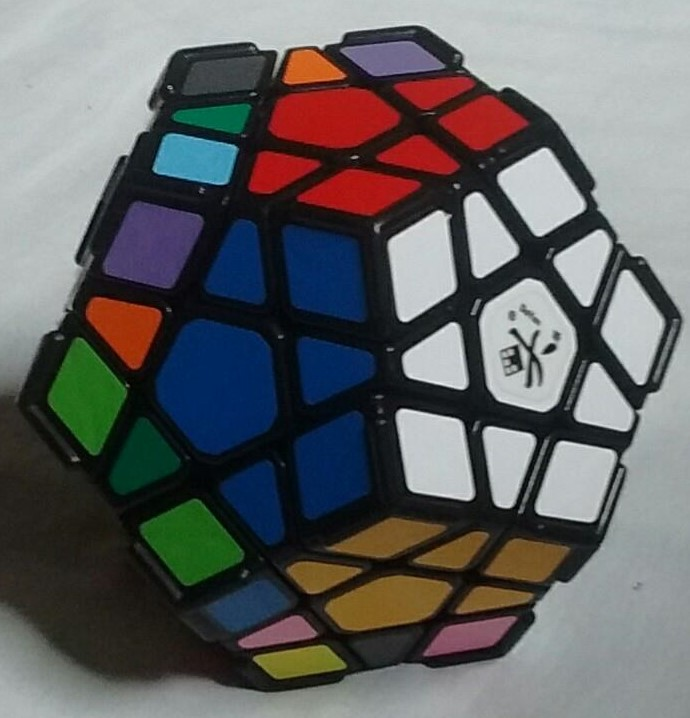
\includegraphics[height=3cm]{imagens/megaminx.jpg}
        \label{figmega}
    }
    \quad %espaco separador
    \subfloat[Pyraminx]{
        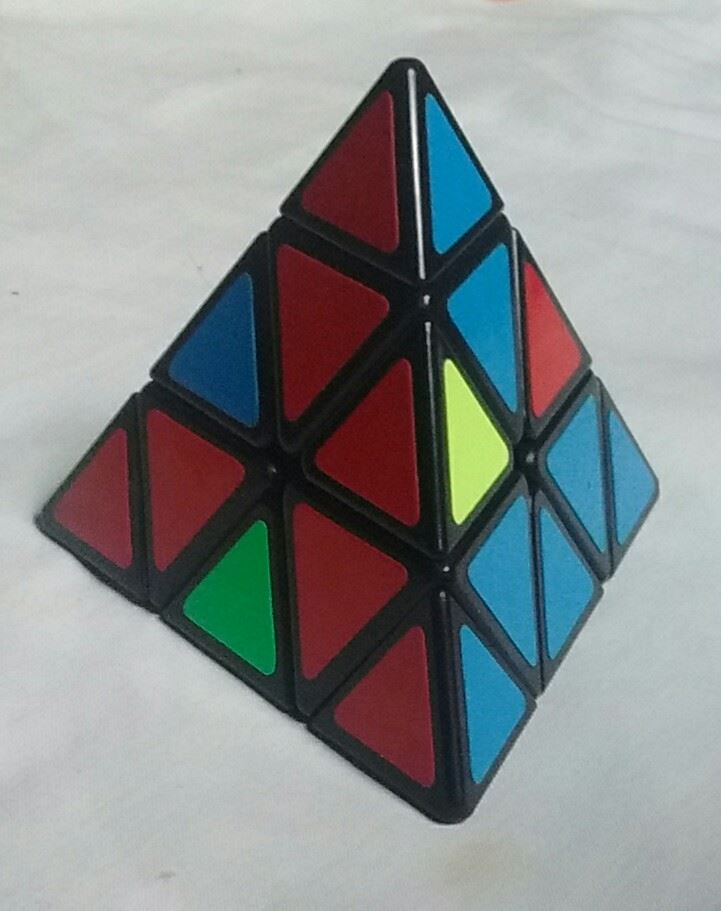
\includegraphics[height=3cm]{imagens/pyraminx.jpg}
        \label{figpyra}
    }
    \quad %espaco separador
    \subfloat[Cubo 2x2x2]{
        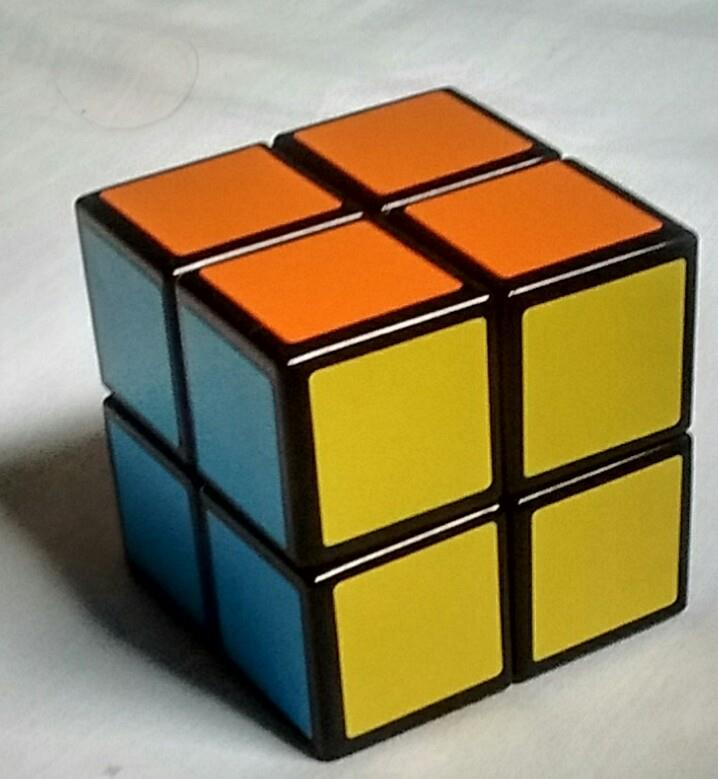
\includegraphics[height=3cm]{imagens/2.jpg}
        \label{fig2}
    }
\caption{Puzzles}
\label{fig:figPuzzles}
\legend{Fonte: Elaborado pelo autor (2017)}
\end{figure}


No campo da ciência da computação, o cubo mágico é caracterizado como um desafio que vai além da simples resolução do quebra-cabeça. Ela está preocupada, dentre outras coisas, com a análise do tempo necessário para a execução dos algoritmos, levando em consideração o número de elementos sobre o qual o algoritmo atua \cite{hardesty}.
A Teoria da Computação levanta alguns questionamentos como, por exemplo, a análise de bons algoritmos e a complexidade na otimização do número de movimentos \cite{erik}. 

\section{Relações envolvendo Teoria dos Grupos}

Matemáticos estudaram o funcionamento do cubo de Rubik na tentativa de sistematizar um método para resolvê-lo e perceberam que seus movimentos ilustram aspectos interessantes de teorias matemáticas \cite{cinoto}. Suas ações e movimentos são elementos que atendem a todas as condições da estrutura de um grupo, assim como também se relacionam com um grupo de permutações \cite{luis}. A essência por trás da Teoria dos Grupos é tomar dois elementos de um conjunto, combinar eles de alguma maneira e retornar um terceiro elemento do mesmo conjunto \cite{galdino}.


\subsection{Grupo de Rubik}
Considerando que R, L, F, B, U e D são os movimentos de 90º no sentido horário das faces direita, esquerda, frente, trás, cima e baixo, respectivamente, o conjunto de todos os movimentos permitidos no cubo chamamos de Grupo \textit{R} de Rubik \cite{luis}. Conforme veremos a seguir, o cubo de Rubik satisfaz as condições para a definição de grupo:

\begin{itemize}
    \item Associatividade: quando realizamos uma sequência qualquer de movimentos, por exemplo, três movimentos genéricos
X, Y e Z, verificamos que: X(Y Z) = (X Y)Z. Ao manipular o cubo a prova desta condição é evidente \cite{luis}.

    \item Elemento neutro: a existência do elemento neutro é verificada pelo movimento "não fazer nada" em qualquer das 6 faces. Com isso garantimos a identidade \textit{I} de qualquer uma das seis faces do cubo ou de qualquer sequência de movimentos \cite{luis}.
    
    \item Elemento inverso: o elemento inverso no Grupo \textit{R} de Rubik significa desfazer a sequência de movimentos. Por exemplo, seja X um movimento qualquer, ou seja, uma rotação de 90º no sentido horário em uma das seis faces, então seu elemento inverso será o movimento, também de 90º, na mesma face, porém no sentido anti-horário. Caso seja efetuado uma sequência de movimentos, então o elemento inverso será a realização dos inversos dos movimentos, porém na ordem inversa.
\end{itemize}


\section{Notações} 

Antes de descrever os métodos de resolução, é essencial definir alguns conceitos e nomenclaturas.


\subsection{Face} 
A \abrv[WCA -- World Cube Association]{WCA}é o órgão que regula as competições de cubo mágico no mundo. Ela estabelece uma notação oficial para cada uma das seis faces do tradicional cubo 3x3x3, onde cada uma é representada por uma letra: F (frente), L (esquerda), R (direita), B (trás), U (topo) e D (inferior).



\begin{figure}[!htb]
    \centering
    \subfloat[Face F]{
        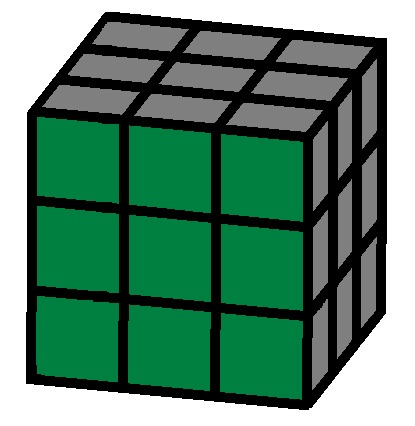
\includegraphics[height=2cm]{imagens/front.jpg}
        \label{figFront}
    }
    \quad %espaco separador
    \subfloat[Face R]{
        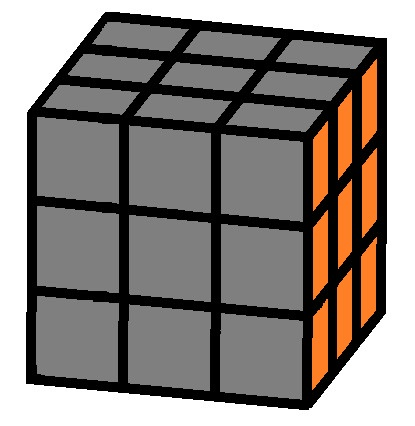
\includegraphics[height=2cm]{imagens/right.jpg}
        \label{figright}
    }
    \quad %espaco separador
    \subfloat[Face U]{
        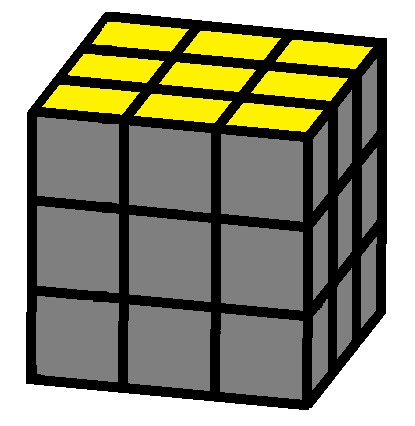
\includegraphics[height=2cm]{imagens/top.jpg}
        \label{figtop}
    }
\caption{Faces}
\label{fig:figFaces}
\legend{Fonte: Elaborado pelo autor (2017)}
\end{figure}

\subsection{Peça} 
Cada peça do quebra-cabeça é formada pelas cores das faces que a compõe. Um exemplo é a peça de meio que pertence às faces F e R, denominada de FR ou RF.

\begin{figure}[!htb]
    \centering
    {
        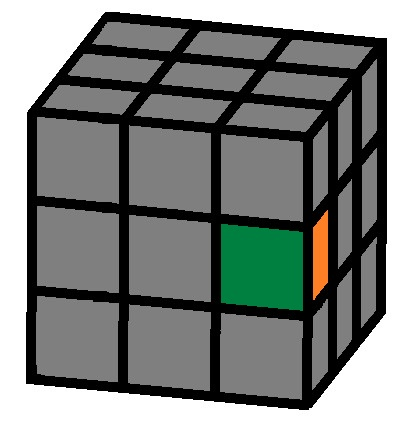
\includegraphics[height=2cm]{imagens/pecaRF.jpg}
        \label{figFront}
    }
    
\caption{Peça FR}
\label{fig:figPeca}
\legend{Fonte: Elaborado pelo autor (2017)}
\end{figure}

O cubo mágico é composto por três tipos de peças. Uma delas é a peça de centro, que é fixa e indica a cor de determinada face. As outras são a peça de meio, que tem duas cores, e a quina, composta por três cores, como mostra a Figura \ref{fig:figPecas}. É importante notar que as peças só podem ser posicionadas no lugar de peças de mesmo tipo.


\begin{figure}[!htb]
    \centering
    \subfloat[Centros]{
        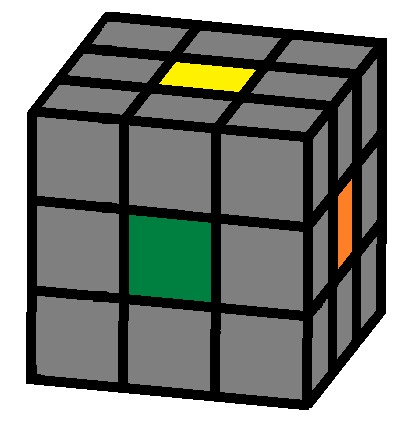
\includegraphics[height=2cm]{imagens/centros.jpg}
        \label{figcentro}
    }
    \quad %espaco separador
    \subfloat[Meios]{
        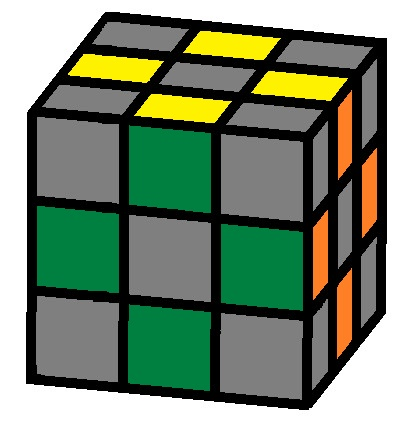
\includegraphics[height=2cm]{imagens/meios.jpg}
        \label{figmeios}
    }
    \quad %espaco separador
    \subfloat[Quinas]{
        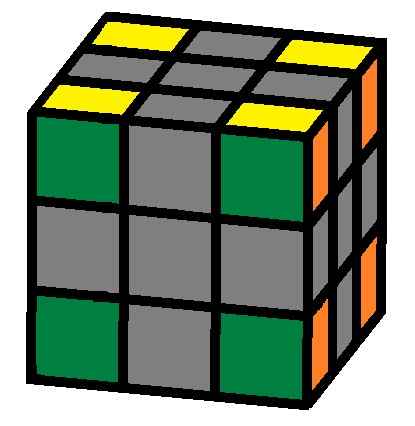
\includegraphics[height=2cm]{imagens/quinas.jpg}
        \label{figquinas}
    }
\caption{Tipos de peças}
\label{fig:figPecas}
\legend{Fonte: Elaborado pelo autor (2017)}
\end{figure}


\subsection{Movimentos} 
Cada face produz três tipos de movimentos básicos: o giro de 90º no sentido horário, de 180º e de 90º no sentido anti-horário. A representação desses giros é feita utilizando a seguinte simbologia: se for um giro de 90º no sentido horário escrevemos apenas a letra que corresponde a face girada; para o giro de 180º colocamos a letra acrescido do número 2; e para o giro de 90º no sentido anti-horário escrevemos a letra mais ‘ (apóstrofo). Por exemplo, a face U produz os seguintes giros: U, U2 e U’, como mostrado na Figura \ref{fig:figGiros}.


\begin{figure}[!htb]
    \centering
    \subfloat[U]{
        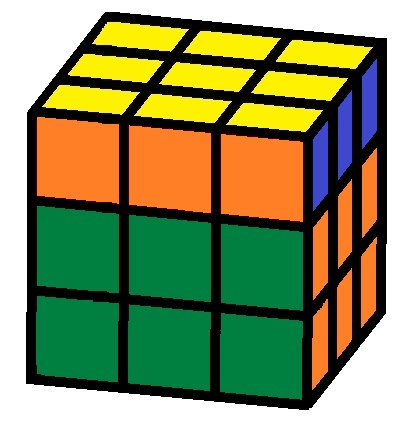
\includegraphics[height=2cm]{imagens/topClock.jpg}
        \label{figcentro}
    }
    \quad %espaco separador
    \subfloat[U2]{
        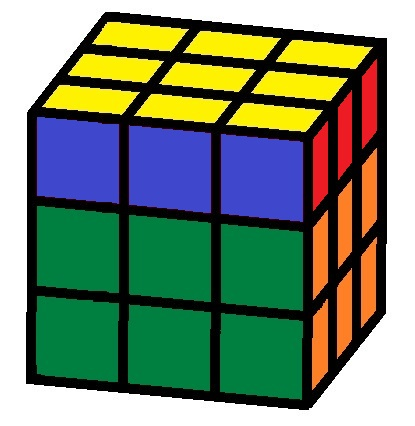
\includegraphics[height=2cm]{imagens/topClock180.jpg}
        \label{figmeios}
    }
    \quad %espaco separador
    \subfloat[U']{
        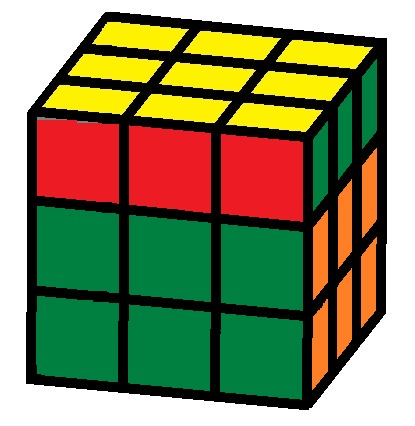
\includegraphics[height=2cm]{imagens/topIClock.jpg}
        \label{figquinas}
    }
\caption{Giros}
\label{fig:figGiros}
\legend{Fonte: Elaborado pelo autor (2017)}
\end{figure}


\subsection{Permutação e Orientação de Peças} 
O conceito de permutação está relacionado ao posicionamento das peças em um estado específico que se encontra o cubo mágico. Nada mais é do que a troca de uma peça por outra. Já a orientação ocorre quando a peça está na sua posição correta, mas ainda assim o cubo não está resolvido.






\section{Métodos de resolução}


O cubo de Rubik possui exatamente  43 252 003 274 489 856 000 combinações possíveis e desde a década de 80 esse quebra-cabeça tridimensional desafia várias pessoas a encontrarem uma solução. Há uma infinidade de maneiras para resolvê-lo. Algumas pessoas solucionam sem auxílio de técnicas. No entanto, essa é uma prática trabalhosa e cansativa e muito mais difícil do que apenas seguir os passos que são dados nos métodos.


Ao aprender um algoritmo, é essencial fazer a repetição dos movimentos e compreender qual o objetivo de cada passo até que se torne algo natural e intuitivo. Os métodos vão desde os mais simples até os mais complexos, isso influencia o tempo que será gasto na solução. Algumas sequências são derivadas de outros métodos ou até mesmo são combinações de vários deles. A seguir será exposto alguns dos métodos mais usados na resolução do cubo de Rubik.

\subsection{Método em Camadas}

O método em camadas é uma das técnicas mais utilizadas na resolução do cubo mágico. Foi inventado em 1979 pelo americano David Singmaster e é conhecida por ser  bastante simples e por não apresentar grande complexidade. Após ganhar seu primeiro cubo mágico, Singmaster demorou cerca de duas semanas para resolvê-lo. Ele elaborou sua própria notação para registrar os movimentos gerados e em junho de 1979 publicou seu primeiro artigo sobre o cubo no jornal The Observer, tornando-se um dos fomentadores do cubo mágico na década de 80. 



Nessa técnica o cubo é dividido em três camadas, como mostra a Figura \ref{fig:figconceiCa}. Para solucioná-las, existem sete passos que devem ser seguidos.


\begin{figure}[!htb]
    \centering
    {
        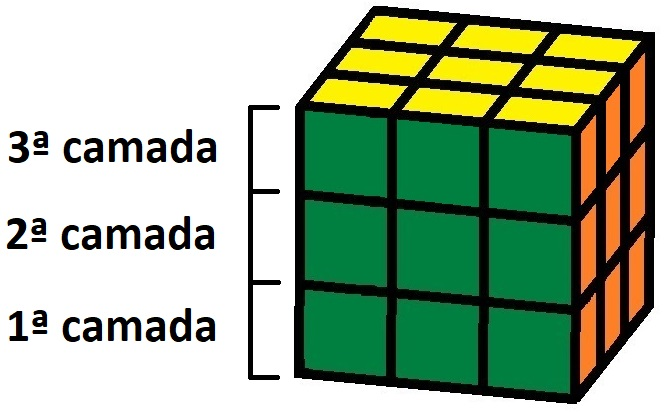
\includegraphics[height=2.5cm]{imagens/conceitoCamadas.jpg}
        \label{figFront}
    }
    
\caption{Divisão em camadas}
\label{fig:figconceiCa}
\legend{Fonte: Elaborado pelo autor (2017)}
\end{figure}


    \subsubsection{1ª etapa}

    O primeiro passo é fazer a cruz na face D. Nessa etapa é importante respeitar as peças de centro, conforme mostrado na Figura \ref{fig:figcc}.
    
    
    
\begin{figure}[!htb]
    \centering
    \subfloat[Correto]{
        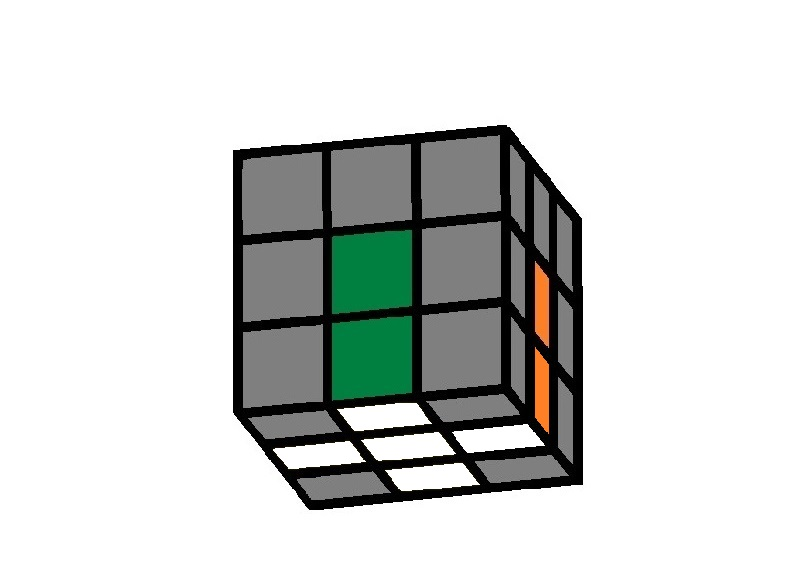
\includegraphics[height=3.3cm]{imagens/centroscorreto.jpg}
        \label{figcentro}
    }
    \quad %espaco separador
    \subfloat[Incorreto]{
        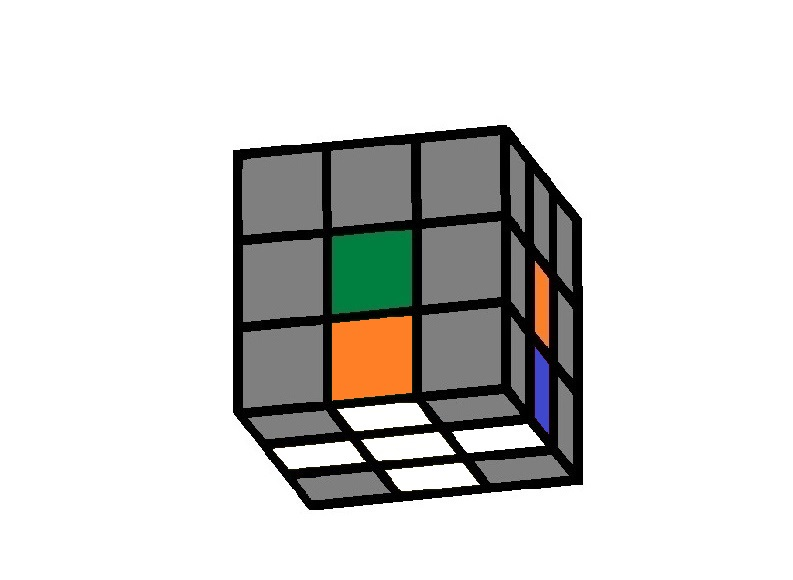
\includegraphics[height=3.3cm]{imagens/centrosincorretos.jpg}
        \label{figmeios}
    }
\caption{Cruz na face D}
\label{fig:figcc}
\legend{Fonte: Elaborado pelo autor (2017)}
\end{figure}
    
    
Embora exista um algoritmo, a construção da cruz é bastante intuitiva, ou seja, com uma simples observação pode-se construí-la sem dificuldades \cite{jose}.  


\subsubsection{2ª etapa}


O objetivo dessa etapa é concluir a primeira camada do cubo mágico, como é mostrado na Figura \ref{fig:fig2222}. Temos quatro peças de meio em seu devido lugar e queremos colocar as outras quatro peças de quina para completar uma face e poder passar ao passo seguinte \cite{jose}. Geralmente aplica-se um único algoritmo nessa etapa que é utilizado para posicionar todas as peças de quina da face D.
\begin{figure}[!htb]
    \centering
    {
        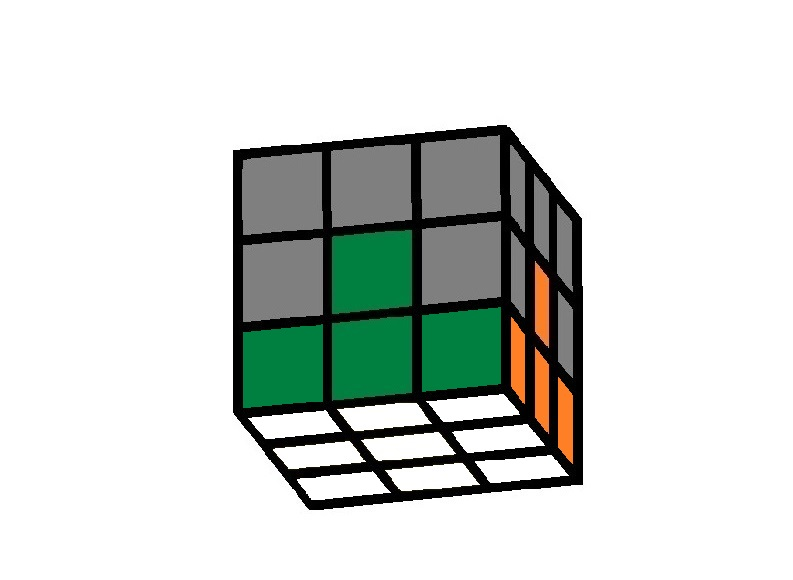
\includegraphics[height=3.3cm]{imagens/passo2.jpg}
        \label{figFront}
    }
    
\caption{Conclusão da primeira camada}
\label{fig:fig2222}
\legend{Fonte: Elaborado pelo autor (2017)}
\end{figure}

\subsubsection{3ª etapa}

O objetivo desse passo é completar a segunda camada, como ilustra a Figura \ref{fig:figpassoo3}. É necessário procurar por peças de meio no topo do cubo e localizar o lugar que ela deverá entrar, respeitando seus centros correspondentes e posicionando-os através da aplicação de um único algoritmo.

\begin{figure}[!htb]
    \centering
    {
        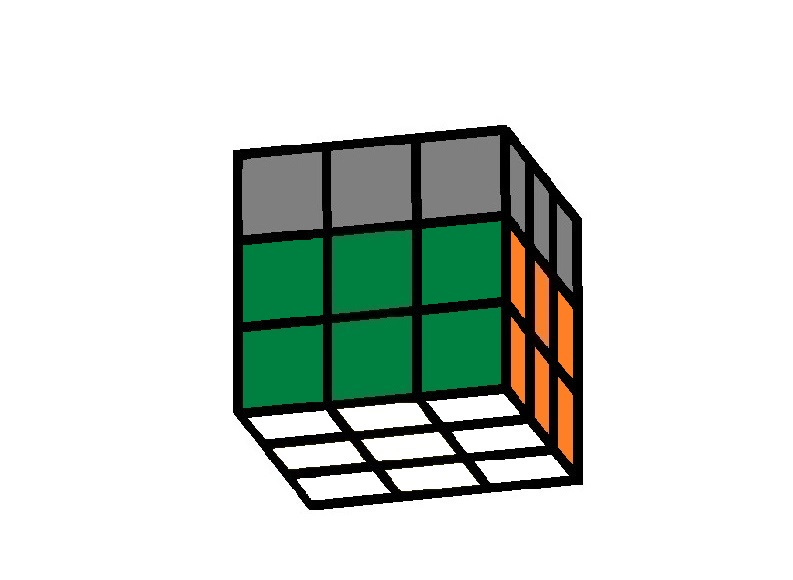
\includegraphics[height=3.3cm]{imagens/passo3.jpg}
        \label{figFront}
    }
    
\caption{Conclusão da segunda camada}
\label{fig:figpassoo3}
\legend{Fonte: Elaborado pelo autor (2017)}
\end{figure}

\subsubsection{4ª etapa}

O objetivo do quarto passo é construir uma cruz na face U, conforme é mostrado na Figura \ref{fig:figpasso4}. É um passo relativamente simples, tendo como fator determinante para sua realização com êxito a forma como o cubo está posicionado antes de se iniciar os movimentos, bastando apenas aplicar o algoritmo correspondente. Como o método tradicional em camadas aplica um único algoritmo em cada etapa, às vezes é necessário repetir o mesmo algoritmo para que as peças sejam posicionadas no lugar correto. 


\begin{figure}[!htb]
    \centering
    {
        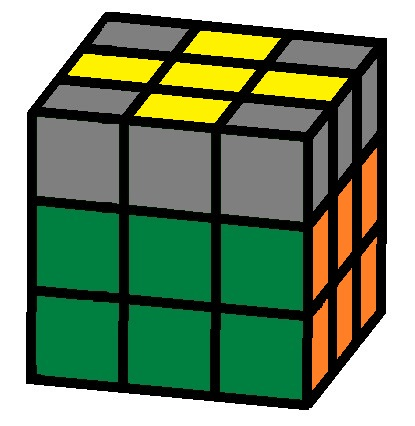
\includegraphics[height=2.4cm]{imagens/passo4.jpg}
        \label{figFront}
    }
    
\caption{Cruz na face U}
\label{fig:figpasso4}
\legend{Fonte: Elaborado pelo autor (2017)}
\end{figure}

\subsubsection{5ª etapa}

Nessa etapa é feita a orientação das peças de quina da face do topo, ou seja, a face do topo é finalizada, como mostrado na Figura \ref{fig:figpasso5}. O cubo pode estar em sete posições diferentes, em qualquer um desses casos o algoritmo será o mesmo, variando apenas a quantidade de vezes que ele será aplicado.

\begin{figure}[!htb]
    \centering
    {
        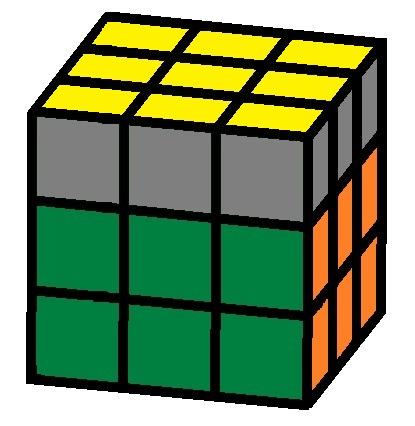
\includegraphics[height=2.4cm]{imagens/passo5.jpg}
        \label{figFront}
    }
    
\caption{Face U finalizada}
\label{fig:figpasso5}
\legend{Fonte: Elaborado pelo autor (2017)}
\end{figure}

\subsubsection{6ª etapa}

A sexta etapa é destinada a permutar as quatro peças de quinas da última camada. Para isso, deve-se encontrar um lado que tenha duas quinas com adesivos de mesma cor, rotacionar o cubo de modo que este lado fique na frente e aplicar o algoritmo correspondente a este passo.

\begin{figure}[!htb]
    \centering
    {
        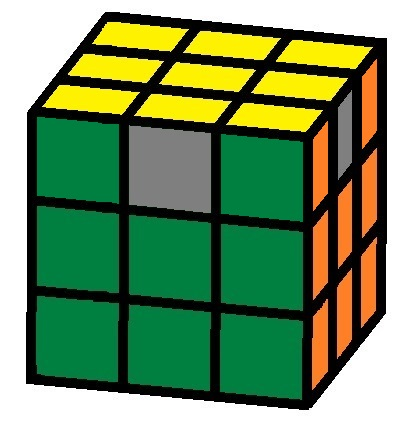
\includegraphics[height=2.4cm]{imagens/passo6.jpg}
        \label{figFront}
    }
    
\caption{Permutação das quinas}
\label{fig:figpasso6}
\legend{Fonte: Elaborado pelo autor (2017)}
\end{figure}

\subsubsection{7ª etapa}

A sétima e última etapa é destinada a permutar as peças de meio. A característica mais marcante desta etapa final é um movimento chamado Minerva, uma alusão à deusa romana das artes e da sabedoria \cite{ana}. A última etapa é mostrada na Figura \ref{fig:figpasso7}, resultando na solução do quebra-cabeça.

\begin{figure}[!htb]
    \centering
    {
        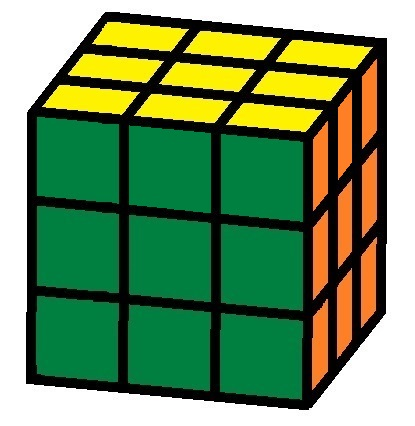
\includegraphics[height=2.4cm]{imagens/passo7.jpg}
        \label{figFront}
    }
    
\caption{Última etapa do método em camadas}
\label{fig:figpasso7}
\legend{Fonte: Elaborado pelo autor (2017)}
\end{figure}


\subsubsection{Avaliação do método em camadas}

Atualmente é o método mais utilizado, principalmente pelo fato de possuir poucos algoritmos, o que facilita a sua memorização. Em alguns casos é necessário repetir o mesmo algoritmo diversas vezes para que o cubo seja solucionado. Evidentemente essa técnica não é a mais eficiente quando analisamos a quantidade de movimentos gerados e o tempo gasto na resolução. Em média esse método realiza 100 movimentos para qualquer configuração do cubo mágico.



\subsection{Método Intermediário}

O método intermediário segue a mesma lógica do método em camadas, porém com alguns algoritmos adicionais. Ele é composto por alguns algoritmos de uma outra solução chamada de método de Fridrich. Sua divisão é feita em seis etapas.

\subsubsection{1ª etapa}
    O objetivo da primeira etapa é resolver a cruz na face D. Este passo é o mesmo do método anterior.
    
\subsubsection{2ª etapa}

Esta etapa destina-se a resolver a primeira camada e, em alguns casos, inserir simultaneamente algumas peças da segunda camada. É a partir desse passo que o método intermediário difere do método em camadas tradicional. São exatamente 10 algoritmos para solucionar a primeira e segunda camada de uma única vez. Este fato torna-o um método um pouco mais complexo do que o anterior. A Figura \ref{fig:intermediario2} ilustra alguns casos possíveis de serem solucionados com os algoritmos definidos dessa etapa.

\begin{figure}[!htb]
    \centering
    \subfloat[Caso 1]{
        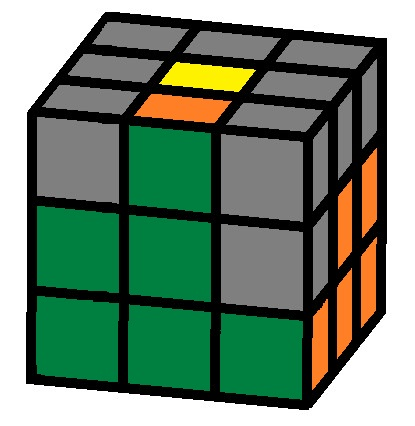
\includegraphics[height=2cm]{imagens/caso1_1.jpg}
        \label{figFront}
    }
    \quad %espaco separador
    \subfloat[Caso 2]{
        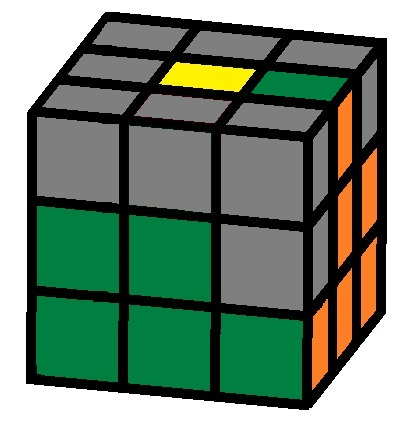
\includegraphics[height=2cm]{imagens/caso2_2.jpg}
        \label{figright}
    }
    \quad %espaco separador
    \subfloat[Caso 3]{
        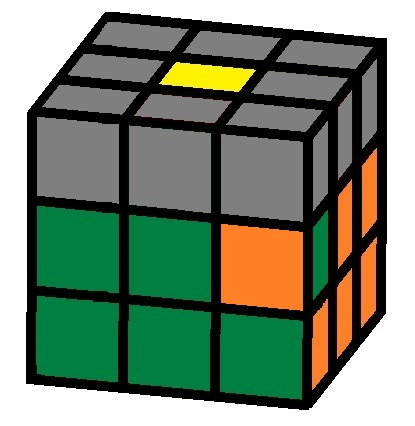
\includegraphics[height=2cm]{imagens/caso3_3.jpg}
        \label{figtop}
    }
\caption{Casos solucionáveis pelo método intermediário - 2ª etapa}
\label{fig:intermediario2}
\legend{Fonte: Elaborado pelo autor (2017)}
\end{figure}

\subsubsection{3ª etapa}

O objetivo desse passo é fazer a cruz na camada U. O método analisa 4 configurações possíveis, como mostra a Figura \ref{fig:intermediariooo3}. Nessa terceira etapa, a probabilidade de o cubo cair diretamente no caso 1, como mostrado na imagem, é de 1/2; no caso 2 é de 1/4; no caso 3 é 1/8; e no caso 4, ou seja, quando a cruz está totalmente feita, não havendo necessidade de aplicar algoritmo, é de 1/8.

\begin{figure}[!htb]
    \centering
    \subfloat[Caso 1]{
        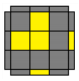
\includegraphics[height=1.8cm]{imagens/c1.png}
        \label{figFront}
    }
    \quad %espaco separador
    \subfloat[Caso 2]{
        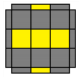
\includegraphics[height=1.8cm]{imagens/c2.png}
        \label{figright}
    }
    \quad %espaco separador
    \subfloat[Caso 3]{
        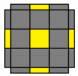
\includegraphics[height=1.8cm]{imagens/c3.png}
        \label{figtop}
    }
    \quad %espaco separador
    \subfloat[Caso 4]{
        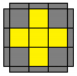
\includegraphics[height=1.8cm]{imagens/c4.png}
        \label{figtop}
    }
\caption{Casos solucionáveis pelo método intermediário - 3ª etapa}
\label{fig:intermediariooo3}
\legend{Fonte: Elaborado pelo autor (2017)}
\end{figure}

\subsubsection{4ª etapa}

O objetivo desse passo, assim como no método anterior, é fazer a orientação das peças de quina da face U. Diferencia-se do método em camadas pelo fato de apresentar 8 casos, ou seja, há 7 algoritmos distintos para solucionar essa etapa. O último caso é quando a face U está completamente resolvida.
	
	
A probabilidade de cair os casos 1, 2, 3, 5, 6 e 7 é de 4/27, e o caso 4 é de 2/27. Já a possibilidade dessa etapa ser desprezada, ou seja, quando o caso 8 é atendido, assim como mostra a Figura \ref{fig:intermediario4}, é de 1/27. 

\begin{figure}[!htb]
    \centering
    \subfloat[Caso 1]{
        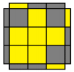
\includegraphics[height=1.8cm]{imagens/cc1.png}
        \label{figFront}
    }
    \quad %espaco separador
    \subfloat[Caso 2]{
        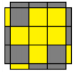
\includegraphics[height=1.8cm]{imagens/cc2.png}
        \label{figright}
    }
    \quad %espaco separador
    \subfloat[Caso 3]{
        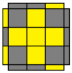
\includegraphics[height=1.8cm]{imagens/cc3.png}
        \label{figtop}
    }
    \quad %espaco separador
    \subfloat[Caso 4]{
        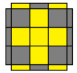
\includegraphics[height=1.8cm]{imagens/cc4.png}
        \label{figtop}
    }
    \quad %espaco separador
    \subfloat[Caso 5]{
        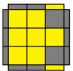
\includegraphics[height=1.8cm]{imagens/cc5.png}
        \label{figright}
    }
    \quad %espaco separador
    \subfloat[Caso 6]{
        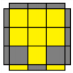
\includegraphics[height=1.8cm]{imagens/cc6.png}
        \label{figtop}
    }
    \quad %espaco separador
    \subfloat[Caso 7]{
        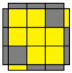
\includegraphics[height=1.8cm]{imagens/cc7.png}
        \label{figtop}
    }
    \quad %espaco separador
    \subfloat[Caso 8]{
        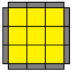
\includegraphics[height=1.8cm]{imagens/cc8.png}
        \label{figtop}
    }
\caption{Casos solucionáveis pelo método intermediário - 4ª etapa}
\label{fig:intermediario4}
\legend{Fonte: Elaborado pelo autor (2017)}
\end{figure}

\subsubsection{5ª etapa}

A penúltima etapa é composta por apenas 3 casos. O primeiro é quando há duas peças de quina de mesma cor na mesma face. Nesse caso, deve rotacionar o cubo de modo que essa face torne-se a face B para em seguida aplicar o algoritmo. A probabilidade de cair o caso 1 é de 2/3. O segundo caso é quando não há peças de quina em um mesmo lado, sua probabilidade é de 1/6. O terceiro e último caso é quando essa etapa é totalmente desprezada, conforme é mostrado no caso 3, tendo 1/6 de chance desse caso ser atendido.

\begin{figure}[!htb]
    \centering
    \subfloat[Caso 1]{
        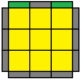
\includegraphics[height=1.8cm]{imagens/ccc1.png}
        \label{figFront}
    }
    \quad %espaco separador
    \subfloat[Caso 2]{
        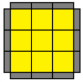
\includegraphics[height=1.8cm]{imagens/ccc2.png}
        \label{figright}
    }
    \quad %espaco separador
    \subfloat[Caso 3]{
        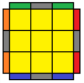
\includegraphics[height=1.8cm]{imagens/ccc3.png}
        \label{figtop}
    }
\caption{Casos solucionáveis pelo método intermediário - 5ª etapa}
\label{fig:intermediario5}
\legend{Fonte: Elaborado pelo autor (2017)}
\end{figure}

\subsubsection{6ª etapa}

A última etapa do método intermediário tem a finalidade de realizar as permutações das peças de meio. São 5 casos, sendo que a probabilidade de ocorrência dos casos 1 e 2 são de 1/3, caso 3 de 1/6 e os casos 4 e 5 de 1/12.

\begin{figure}[!htb]
    \centering
    \subfloat[Caso 1]{
        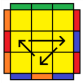
\includegraphics[height=1.8cm]{imagens/cccc1.png}
        \label{figFront}
    }
    \quad %espaco separador
    \subfloat[Caso 2]{
        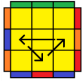
\includegraphics[height=1.8cm]{imagens/cccc2.png}
        \label{figright}
    }
    \quad %espaco separador
    \subfloat[Caso 3]{
        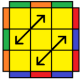
\includegraphics[height=1.8cm]{imagens/cccc3.png}
        \label{figtop}
    }
    \quad %espaco separador
    \subfloat[Caso 4]{
        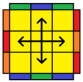
\includegraphics[height=1.8cm]{imagens/cccc4.png}
        \label{figtop}
    }
    \quad %espaco separador
    \subfloat[Caso 5]{
        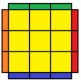
\includegraphics[height=1.8cm]{imagens/cccc5.png}
        \label{figtop}
    }
\caption{Casos solucionáveis pelo método intermediário - 6ª etapa}
\label{fig:intermediario6}
\legend{Fonte: Elaborado pelo autor (2017)}
\end{figure}


\subsubsection{Avaliação do método intermediário}


O método intermediário é uma extensão do método tradicional em camadas. Além de usarem o mesmo conceito de camadas, o intermediário também possui o mesmo conjunto de algoritmos do método anterior.

Na verdade, o método intermediário é uma espécie de transição do método em camadas para o Fridrich \cite{alcantara}, técnica mais avançada que será explicada adiante. Seu diferencial é o fato de ter mais algoritmos para resolver duas camadas ao mesmo tempo. Em outras palavras: essa técnica possui "atalhos" que não há no método tradicional em camadas. Consequentemente o resultado disso é a redução da quantidade total de movimentos realizados e a diminuição do tempo gasto para montar o cubo, um total de 30 a 40 segundos a menos que o método anterior. 



\subsection{Fridrich}

O método de Fridrich, também conhecido como \abrv[CFOP -- Cross, First 2 Layers, Orient Last Layer, Permute Last Layer]{CFOP}pelos competidos do quebra-cabeça, foi desenvolvido pela professora de engenharia elétrica Jessica Fridrich, no qual apresenta 119 fórmulas diferentes, e que permite a resolução do cubo em menos de 1 minuto \cite{alan}. Atualmente é o método avançado mais conhecido e mais utilizado no mundo por quem objetiva diminuir o tempo de solução do cubo de Rubik.

\begin{quotation}
Fridrich decifrou pela primeira vez as faces coloridas do cubo em 1981, quando era uma adolescente vivendo numa cidade tcheca mineradora de carvão. Poucas pessoas passaram décadas decodificando um bloco de plástico, não importa quão matematicamente complicado. Mas poucas pessoas são tão tenazes quanto a arquiteta do Método Fridrich \cite{bina}.
\end{quotation}

Para Fridrich, lidar com um quebra-cabeça dificílimo não era simplesmente um hobby, era obsessão. Impossibilitada de sair da Tchecoslováquia até a Revolução de Veludo, que lhe permitiu migrar para os Estados Unidos e fazer seu doutorado, Fridrich, autodidata em cálculo diferencial e integral, esboçou a solução do quebra-cabeça em um caderno antes mesmo de possuir o brinquedo. Hoje em dia, o cubo não é mais território desconhecido, mas um terreno bastante explorado por computadores pessoais e mãos suadas. \cite{bina}.


O Método Fridrich segue o conceito de camadas, mas, diferentemente do método tradicional, ele resolve as duas primeiras camadas de uma única vez e, diferentemente do método intermediário, é composto por algoritmos mais avançados. A maioria dos "speedcubers", os solucionadores que competem para resolver o cubo no menor espaço de tempo, internalizam o método usando apenas a intuição. 

Este método é grande e trabalhoso, porém, o resultado é excelente \cite{renann}. Seu diferencial está no fato de contemplar mais casos do que os métodos anteriores. Adiante são mostrados os passos para solucionar o cubo utilizando o método de Fridrich.

\subsubsection{1ª etapa}

A primeira etapa do Fridrich é a mesma realizada nos dois métodos anteriores. Geralmente esse passo é resolvido de maneira totalmente intuitiva, dado que, por se tratar de um método avançado, subentende-se que esse passo seja resolvido de maneira rápida e sem dificuldades pelas pessoas que já estão habituadas com essa técnica. Para formar a cruz na face D são realizados, em média, 6 movimentos ou menos.


\subsubsection{2ª etapa}


É nesse ponto que o Fridrich se diferencia do método intermediário. Na verdade, os 10 casos que englobam a 2ª etapa do método intermediário foram herdados do Fridrich. A diferença é que, no Fridrich, há exatamente 31 casos a mais do que o método anterior, totalizando 41 casos.

Seu objetivo é resolver as duas primeiras camadas simultaneamente, reduzindo consideravelmente o tempo de resolução. Essa etapa é frequentemente chamada de \abrv[F2L -- First two layers]{F2L}pelos utilizadores dessa técnica. Normalmente esse conjunto de algoritmos é dividido em grupos, afim de facilitar a sua memorização, conforme é mostrado na Tabela 1. A segunda coluna da tabela informa a quantidade de casos contemplados por cada divisão e a terceira coluna mostra o intervalo da quantidade de movimentos realizado por cada caso.


\begin{table}[!htb]   
    \textsf{\caption{Divisão dos casos F2L}}
    \centering
    \medskip
   
    \begin{tabular}{c|c|c}  
        \hline
        \textbf{Nome} & 
        \textbf{Casos} &
        \textbf{Movimentos} \\
        \hline
        Easy Cases & 4 & De 3 a 4  \\
        \hline
        Reposition Edge & 4 & De 8 a 9  \\
        \hline
        Reposition Edge and Flip Corner & 6 & De 8 a 9  \\
        \hline
        Split Pair by Going Over & 4 & De 7 a 9  \\
        \hline
        Pair Made on Side & 4 & De 8 a 9  \\
        \hline
        Weird & 2 & De 8 a 13 \\
        \hline
        Corner in Place, Edge in U Face & 6 & De 7 a 9 \\
        \hline
        Edge in Place, Corner in U Face & 6 & De 7 a 11 \\
        \hline
        Edge and Corner in Place & 5 & De 11 a 12 \\
        \hline
    \end{tabular}
    \label{table:tab1}
\end{table}


\subsubsection{3ª etapa}

A terceira etapa é comumente chamada de \abrv[OLL -- Orient last layer]{OLL}e tem o objetivo de montar toda a face U. Esse passo contempla todos os casos da 3ª e 4ª etapa do intermediário, além de ter casos adicionais, totalizando 57 algoritmos. Esse é mais um aspecto que o diferencia do método anterior, aumentando ainda mais o seu grau de complexidade e dificuldade de memorização. 
    
    
Assim como na 2ª etapa, os casos da OLL também são divididos em grupos, como mostrado na Tabela 2.


\begin{table}[!htb]   
    \textsf{\caption{Divisão dos casos OLL}}
    \centering
    \medskip
   
    \begin{tabular}{c|c|c}  
        \hline
        \textbf{Nome} & 
        \textbf{Casos} &
        \textbf{Movimentos} \\
        \hline
        All Edges Oriented Correctly & 7 & De 7 a 14  \\
        \hline
        Corners Correct, Edges Flipped & 2 & De 7 a 9  \\
        \hline
        P-Shapes & 4 & De 6 a 10  \\
        \hline
        W-Shapes & 2 & 12 \\
        \hline
        Squares & 2 & 7 \\
        \hline
        L Shapes & 6 & De 9 a 12 \\
        \hline
        Fish Shapes & 4 & De 9 a 12 \\
        \hline
        Awkward Shapes & 4 & De 11 a 15 \\
        \hline
        Lightning Bolts & 6 & De 9 a 13 \\
        \hline
        T-Shapes & 2 & De 6 a 8 \\
        \hline
        C-Shapes & 2 & De 8 a 12 \\
        \hline
        I Shapes & 4 & De 10 a 12 \\
        \hline
        Knight Move Shapes & 4 & De 10 a 11 \\
        \hline
        No Edges Flipped Correctly & 8 & De 11 a 13 \\
        \hline
    \end{tabular}
    \label{table:tab2}
\end{table}
    
\subsubsection{4ª etapa}

A última etapa do Fridrich é chamado de \abrv[PLL -- Permutation last layer]{PLL}e é destinada a permutar todas as peças da face U, ou seja, posicionar cada uma no seu devido lugar utilizando apenas um dos 21 casos. Os casos da 6ª etapa do intermediário também estão incluídos aqui. A Tabela 3 apresenta a divisão dos casos e o intervalo de movimentos.


\begin{table}[!htb]   
    \textsf{\caption{Divisão dos casos PLL}}
    \centering
    \medskip
   
    \begin{tabular}{c|c|c}  
        \hline
        \textbf{Nome} & 
        \textbf{Casos} &
        \textbf{Movimentos} \\
        \hline
        Permutations of Edges or Corners Only & 7 & De 8 a 17 \\
        \hline
        Swap One Set of Adjacent Corners  & 6 & De 11 a 15 \\
        \hline
        Swap One Set of Corners Diagonally  & 4 & De 14 a 18  \\
        \hline
        Double Spins  & 4 & 13  \\
        \hline
    \end{tabular}
    \label{table:tab2}
\end{table}


\subsubsection{Avaliação do Fridrich}

Evidentemente o método Fridrich é mais avançado do que os outros apresentados anteriormente, não é à toa que ele é utilizado pelos principais competidores de cubo mágico no mundo. Apesar de incluir todos os casos presentes no método intermediário, o seu principal diferencial é o fato de introduzir novos algoritmos que visam reduzir ainda mais o número de movimentos e o tempo gasto na resolução do quebra-cabeça. 


O ponto negativo é que, em razão da grande quantidade de casos, a memorização é demorada. Para facilitar, é necessário fazer repetidas vezes os mesmos movimentos e procurar entender o objetivo de cada algoritmo, de modo que vire algo intuitivo.

\subsection{Método Petrus}

Assim como o Fridrich, o método de Lars Petrus, conhecido como Petrus, também é considerado avançado.


\begin{quotation}
Seu criador, Lars Petrus, consagrou-se como um "speedcuber" conhecido internacionalmente depois que ganhou o Campeonato Nacional da Suécia em 1981 e ficou em quarto lugar no Campeonato Mundial de Budapeste em 1982. Mais tarde, Petrus publicou o método conhecido como o método de Petrus, tornando-se um método extremamente popular entre os "cubistas" intermediários e avançados \cite{ignacio}.
\end{quotation}


A grande diferença entre este método e os outros explicados anteriormente é que ele não se baseia no conceito de camadas, e sim no conceito de blocos, como mostra a Figura \ref{fig:figconcesdadadasdiBlo}.


\begin{figure}[!htb]
    \centering
    {
        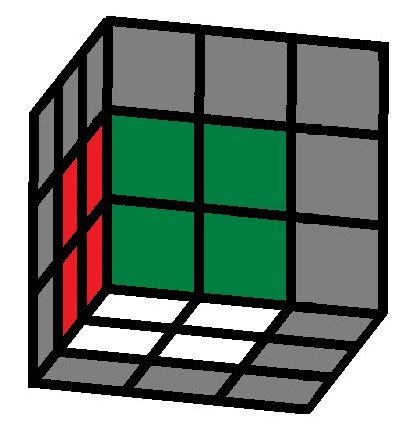
\includegraphics[height=2.4cm]{imagens/conceitoBloco.jpg}
        \label{figFront}
    }
    
\caption{Conceito de blocos}
\label{fig:figconcesdadadasdiBlo}
\legend{Fonte: Elaborado pelo autor (2017)}
\end{figure}



Nessa técnica não existe uma sequência de movimentos pré-definidas que devem ser seguidas para se atingir um resultado esperado. O que há é a ideia básica por trás da solução, ou seja, a solução do cubo mágico é efetuada de maneira totalmente intuitiva, através da ideia de construção de blocos. 

\subsubsection{Avaliação da solução}

Em determinadas configurações do cubo mágico, essa solução pode se tornar mais vantajosa que o Fridrich, em razão de otimizar a solução através da construção de blocos. No entanto, é notório que essa técnica apresenta um maior nível de dificuldade quando comparada ao método de Fridrich, especialmente para os cubistas iniciantes e intermediários. Isso pode ser concluído principalmente pelo fato da solução apresentar uma grande quantidade de movimentos intuitivos. Consequentemente essa solução torna-se difícil quando se deseja trabalhar na otimização do tempo e da movimentação.



\section{Avaliação geral}


Após a avaliação das quatro soluções, é evidente que o entendimento dos mecanismos do cubo de Rubik tornam-se mais simples e fáceis utilizando o conceito de camadas. Dentre todos as técnicas apresentadas, três utilizam esse conceito: método tradicional em camadas, método intermediário e o método de Fridrich.


A solução do tradicional método em camadas é a mais simples, pois apresenta poucos algoritmos e os poucos casos contemplados por ela são suficientes para resolver o problema do cubo mágico em um tempo razoável e realizando uma média 100 movimentos. Já o método intermediário é relativamente simples, porém é apenas uma solução introdutória ao método de Fridrich, que é mais avançado e apresenta mais algoritmos, resultando em uma solução otimizada para qualquer configuração inicial do cubo mágico.

Com isso, as soluções escolhidas para serem implementadas e analisadas mais detalhadamente no decorrer deste trabalho é o método tradicional em camadas e o método de Fridrich.
